\documentclass[11pt,letterpaper]{article}

\input{../../../../.config/latex/preamble_v1.tex}
\lightmode

\title{\textbf{Math 129 Problem Set 1}}

\begin{document}
\maketitle

% Problem 1
\begin{cproblem}{1.7}
  Show that $\Z[i]$ is a principal ideal domain. 
\end{cproblem}

\begin{solution}
  Let $I\subset \Z[i]$ be an ideal. Suppose $\alpha\in I-\{0\}$ is some nonzero element with minimal norm, i.e. every other element in the ideal has norm greater than or equal to $\alpha$. Now consider the $\Z$-lattice generated by $\alpha$ in $\Z[i]$, i.e. $\alpha\Z[i]=(\alpha)$. We claim that this lattice is the entire ideal itself, i.e. $I=(\alpha)$. Suppose there is some Gaussian integer $\omega\not\in (\alpha)$ outside the lattice. Since the lattice covers the whole space, it must fall into one of the lattice squares. Pick the nearest lattice neighbor to $\omega$, say it is $\nu\alpha$ for some $\nu\in \Z[i]$.  
  \begin{figure}[ht]
    \centering
    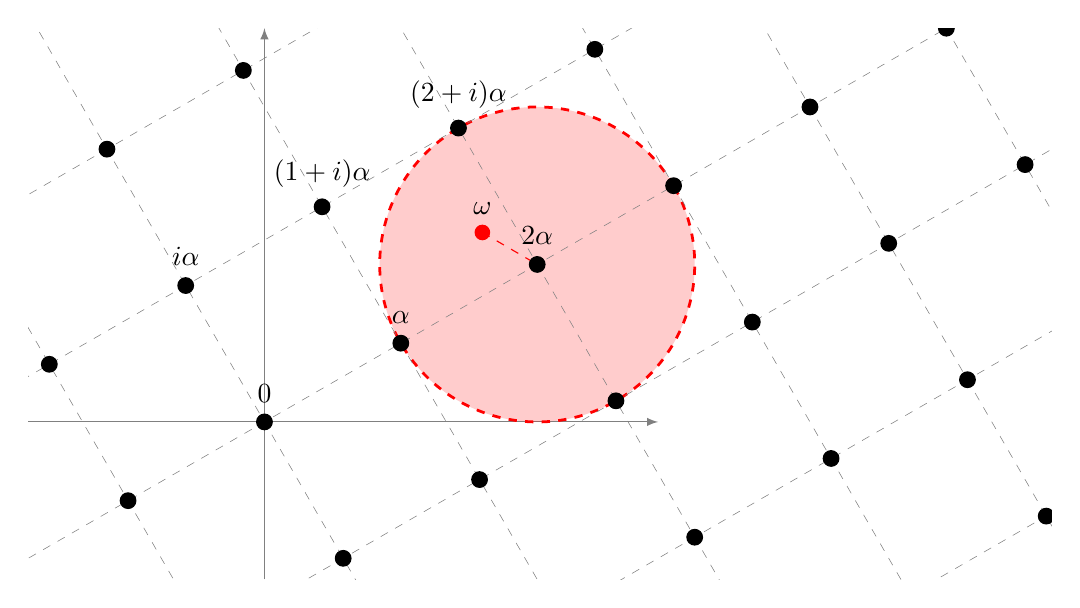
\begin{tikzpicture}
      \coordinate (Origin)   at (0,0);
      \coordinate (XAxisMin) at (-3,0);
      \coordinate (XAxisMax) at (5,0);
      \coordinate (YAxisMin) at (0,-2);
      \coordinate (YAxisMax) at (0,5);
      \draw [thin, gray,-latex] (XAxisMin) -- (XAxisMax);% Draw x axis
      \draw [thin, gray,-latex] (YAxisMin) -- (YAxisMax);% Draw y axis
  
      \clip (-3,-2) rectangle (10cm,5cm); % Clips the picture...
      \pgftransformrotate{30}
      \coordinate (Bone) at (0,2);
      \coordinate (Btwo) at (2,-2);
      \filldraw[fill=red, fill opacity = 0.2, draw=red,dashed,line width=1pt] (4,0) circle (2);
      % Draw outlier point
      \draw [thin, red, dashed] (3.6,0.7) -- (4,0);
      \node[fill=red, circle, inner sep=2pt, label={$\omega$}] at (3.6, 0.7) {};
      \draw[style=help lines,dashed] (-14,-14) grid[step=2cm] (14,14);
      \foreach \x in {-7,-6,...,7}{% Two indices running over each
        \foreach \y in {-7,-6,...,7}{% node on the grid we have drawn 
          \node[draw,circle,inner sep=2pt,fill] at (2*\x,2*\y) {};
        }
      }
      \node[label={$\alpha$}] at (2,0) {};
      \node[label={$2\alpha$}] at (4,0) {};
      \node[label={$(1+i)\alpha$}] at (2,2) {};
      \node[label={$(2+i)\alpha$}] at (4,2) {};
      \node[label={$i\alpha$}] at (0, 2) {};
      \node[label={$0$}] at (0,0) {};
      
    \end{tikzpicture}
    \caption{Lattice generated by $\alpha$} 
  \end{figure}
  
  Then $0<\mathcal{N}(\omega-\nu \alpha) < \mathcal{N}(\alpha)$, since $\omega$ is always contained in a radius $\mathcal{N}(\alpha)$ circle centered at the closest Gaussian integer. This is a contradiction to the norm minimality of $\alpha$, hence $\omega\in (\alpha)$ and so the ideal is principal.  
\end{solution}

% Problem 2
\begin{cproblem}{1.15}
  Here is a proof of Fermat's conjecture for $n=4$:
  \medskip
  \begin{solution} If $x^4+y^3=z^4$ has a solution in positive integers, then so does $x^4+y^4=w^2$. Let $x,y, w$ be a solution with smallest possible $w$. Then $x^2, y^2, w$ is a primitive Pythagorean triple. Assuming (without loss of generality) that $x$ is odd, we can write
  \[
    x^2=m^2-n^2, \quad y^2=2mn, \quad w=m^2+n^2
  \]
  with $n$ and $m$ relative prime positive integers, not both odd. \end{solution}
  \begin{enumerate}[(a)]
    \item Show that
    \[
      x=r^2-s^2, \quad n=2rs,\quad m=r^2+s^2
    \]
    with $r$ and $s$ relative prime positive integers, not both odd.
    \item Show that $r,s,$ and $m$ are pairwise relative prime. Using $y^2=4rsm$, conclude that $r, s,$ and $m$ are all squares, say $a^2, b^2$, and $c^2$.
    \item Show that $a^4+b^4=c^2$, and that this contradicts minimality of $w$.       
  \end{enumerate}     
\end{cproblem}

\begin{solution}
  \textbf{(a)} Note that since $x^2+n^2=m^2$, there must exist integers $r,s$ such that 
  \[
    x=r^2-s^2, \quad n=2rs,\quad m=r^2+s^2
  .\]  
  These integers are relatively prime because if a prime $p|r,s$ then $p|x,m,n$, a contradiction since $m,n$ are coprime. One of them must be even since $x$ is odd.      

  \textbf{(b)} We've established that $(r,s)=1$. Now suppose $p|r,m$. Them $p|s$ since $m=r^2+s^2$ so $p|x,m,n$ which is impossible since they are coprime. Next we claim that $r,s,m$ are all squares. Indeed, note that $y^2=4rsm$, and suppose that $p|r$. Then $p|y^2$ so $p^2|4rsm$. Since $r,s,m$ are all coprime, it thus follows that $p^2|r$. 
  
  Note that we can ignore the case when $p=2$ because both $4$ can only add an even number of two's, hence preserving the square property. Since every prime factor appears twice, it follows that $r$ is a square. The same follows for $s,m$.          

  \textbf{(c)} Since $a^2=r$, $b^2=s$, and $c^2=m$, if follows from $m=r^2+s^2$ that $a^4+b^4=c^2$. But $w=c^4+n^2$ so $c < w$, a contradiction. Thus there can be no solution.       
\end{solution}

% Problem 3
\begin{cproblem}{1.16}
  Show that 
  \[
    (1-\omega)(1-\omega^2)\cdots(1-\omega^{p-1})=p.
  \]
\end{cproblem}

\begin{solution}
  We know that 
  \[
    t^{p}-1=(t-1)(t-\omega)(t-\omega^2)\cdots(t-\omega^{p-1}).
  \]
  Factoring $t-1$ out from both sides of an equation yields
  \[
    t^{p-1}+t^{p-2}+\cdots+t+1 = (t-\omega)(t-\omega^2)\cdots(t-\omega^{p-1})
  \] 
  and substituting $t=1$ yields the desired equation.
\end{solution}

% Problem 4
\begin{cproblem}{1.17}
  Suppose $\Z[\omega]$ is a UFD and that $\pi \mid x+y \omega$. Show that $\pi$ does not divide any of the factors $x+y\omega^i$ for $1<i\leq p$. (Note that $x+y=x+y\omega^p$.)   
\end{cproblem}

\begin{solution}
  Recall that 
  \[
    (x+y)(x+y\omega)(x+y \omega^2)\cdots(x+y \omega^{p-1})=z^p.
  \]
  Let $\pi \mid x+y\omega$ be some non unit factor, then we have $\pi \mid z^p$. Next, suppose for the sake of contradiction that $\pi \mid x+y\omega^i$. Then $\pi \mid (x+y\omega) - (x+y\omega^i)$ so $\pi \mid y\omega(1-\omega^{i-1})$. By Problem~3,
  \[
    \pi \mid y\omega(1-\omega)(1-\omega^2)\cdots (1-\omega^{p-1}) = y\omega p,
  \]  
  however since $\omega$ is a unit it follows that $\pi \mid yp$. So $\pi$ divides both $yp$ and $z^p$, which are relatively prime by assumption, and since $p\nmid z$. Thus by Bezout's identity there exist $n,m\in \Z$ such that $ypn+z^pm=1$. However this implies that $\pi \mid 1$, a contradiction since $\pi$ isn't a unit. Hence, the two terms share no common factors.   
\end{solution}

% Problem 5
\begin{cproblem}{1.18}
  Use Problem~1.17 to show that if $\Z[\omega]$ is a UFD then $x+y\omega=u\alpha^p$ for some $\alpha\in \Z[\omega]$, where $u$ is a unit in $\Z[\omega]$.      
\end{cproblem}

\begin{solution}
  Again, since $\Z[\omega]$ is a UFD, it suffices to show that for any prime $\pi \mid x+y\omega$, we have $\pi^p \mid x+y\omega$. Let $\pi\in \Z[\omega]$ be a prime dividing $x+y\omega$. Then $\pi \mid z^p$ so by primality $\pi\mid z$ and hence \[pi^p \mid (x+y)(x+y\omega)(x+y\omega^2)\cdots(x+y\omega^{p-1}).\] However by Problem~1.17, none of the other factors are divisible by $\pi$, so $\pi^p\mid x+y\omega$. By unique factorization, we thus have $x+y\omega = u\alpha^p$ for some unit $u\in \Z[\omega]$.     
\end{solution}

% Problem 6
\begin{cproblem}{1.19}
  Dropping the assumption that $\Z[\omega]$ is a UFD but using the fact that ideals factor uniquely (up to order) into prime ideals, show that the principal ideal $(x+y\omega)$ has no prime ideal factor in common with any other principal ideals on the left side of the equation
  \[
    (x+y)(x+y\omega)\cdots(x+y\omega^{p-1}) = (z)^p
  \]
  in which all factors are interpreted as principal ideals. 
\end{cproblem}

\begin{solution}
   Suppose $\mathfrak{p} \supset (x+y\omega)$ is a prime factor. Then $\mathfrak{p} \supset (z)^p$, so by the definition of a prime ideal $\mathfrak{p} \supset (z)$. Now suppose for the sake of contradiction that $\mathfrak{p}\supset (x+y\omega^i)$. Since $\mathfrak{p} \supset (x+y\omega)$ and $\mathfrak{p} \supset (x+y\omega^i)$, it follows that 
   \[
       \begin{aligned}
        \mathfrak{p} &\supset (x+y\omega, x+y\omega^i) \supset (y\omega(1-\omega^{i-1}))\\&=y(1-\omega^{i-1})\supset y(1-\omega)(1-\omega^2)\cdots(1-\omega^{p-1})\\&=(yp).
       \end{aligned}
    \] 
    Since $\mathfrak{p} \supset (yp)$ and $\mathfrak{p} \supset (z)$, $\mathfrak{p} \supset (z,yp) = \Z[\omega]$ by Bezout's identity. This is a contradiction since $\mathfrak{p}$ is proper.      
\end{solution}

\pagebreak
% Problem 7
\begin{cproblem}{1.20}
   Use Problem~1.19 to show that $(x+y\omega)=I^p$ for some ideal $I$.   
\end{cproblem}

\begin{solution}
   Since $\Z[\omega]$ has unique factorization of ideals, it suffices to show that for any prime ideal $\mathfrak{p} \supset (x+y\omega)$, $\mathfrak{p}^p\supset (x+y\omega)$. Note that if $\mathfrak{p} \supset (x+y\omega)$, then $\mathfrak{p} \supset (z)^p$ so $\mathfrak{p} \supset (z)$ by the definition of a prime ideal. Then 
   \[
       \mathfrak{p}^p \supset (x+y)(x+y\omega)(x+y\omega^2)\cdots(x+y\omega^{p-1})
   ,\]
   however $\mathfrak{p} \not\supset (x+y\omega^i)$ for $i\neq 1$ by Problem~1.19, so $\mathfrak{p}^p\supset (x+y\omega)$. This concludes the proof.          
\end{solution}

\end{document}